\documentclass[12pt,reqno]{amsart}
\usepackage{/Users/johnmyers/GoogleDrive/tex/handout,/Users/johnmyers/GoogleDrive/tex/customcommands,polynom}
\usepackage{caption}

\hdr{MAT 240}{\S12.1 Functions of two variables, part 1}

\begin{document}

\textbf{Suggested problems:} 1-37 odd

\bigskip
\hrule

\bigskip

\prob The temperature adjusted for wind chill is a temperature which tells you how cold it feels, as a result of the combination of wind and temperature; see the table below.

\medskip
\begin{center}
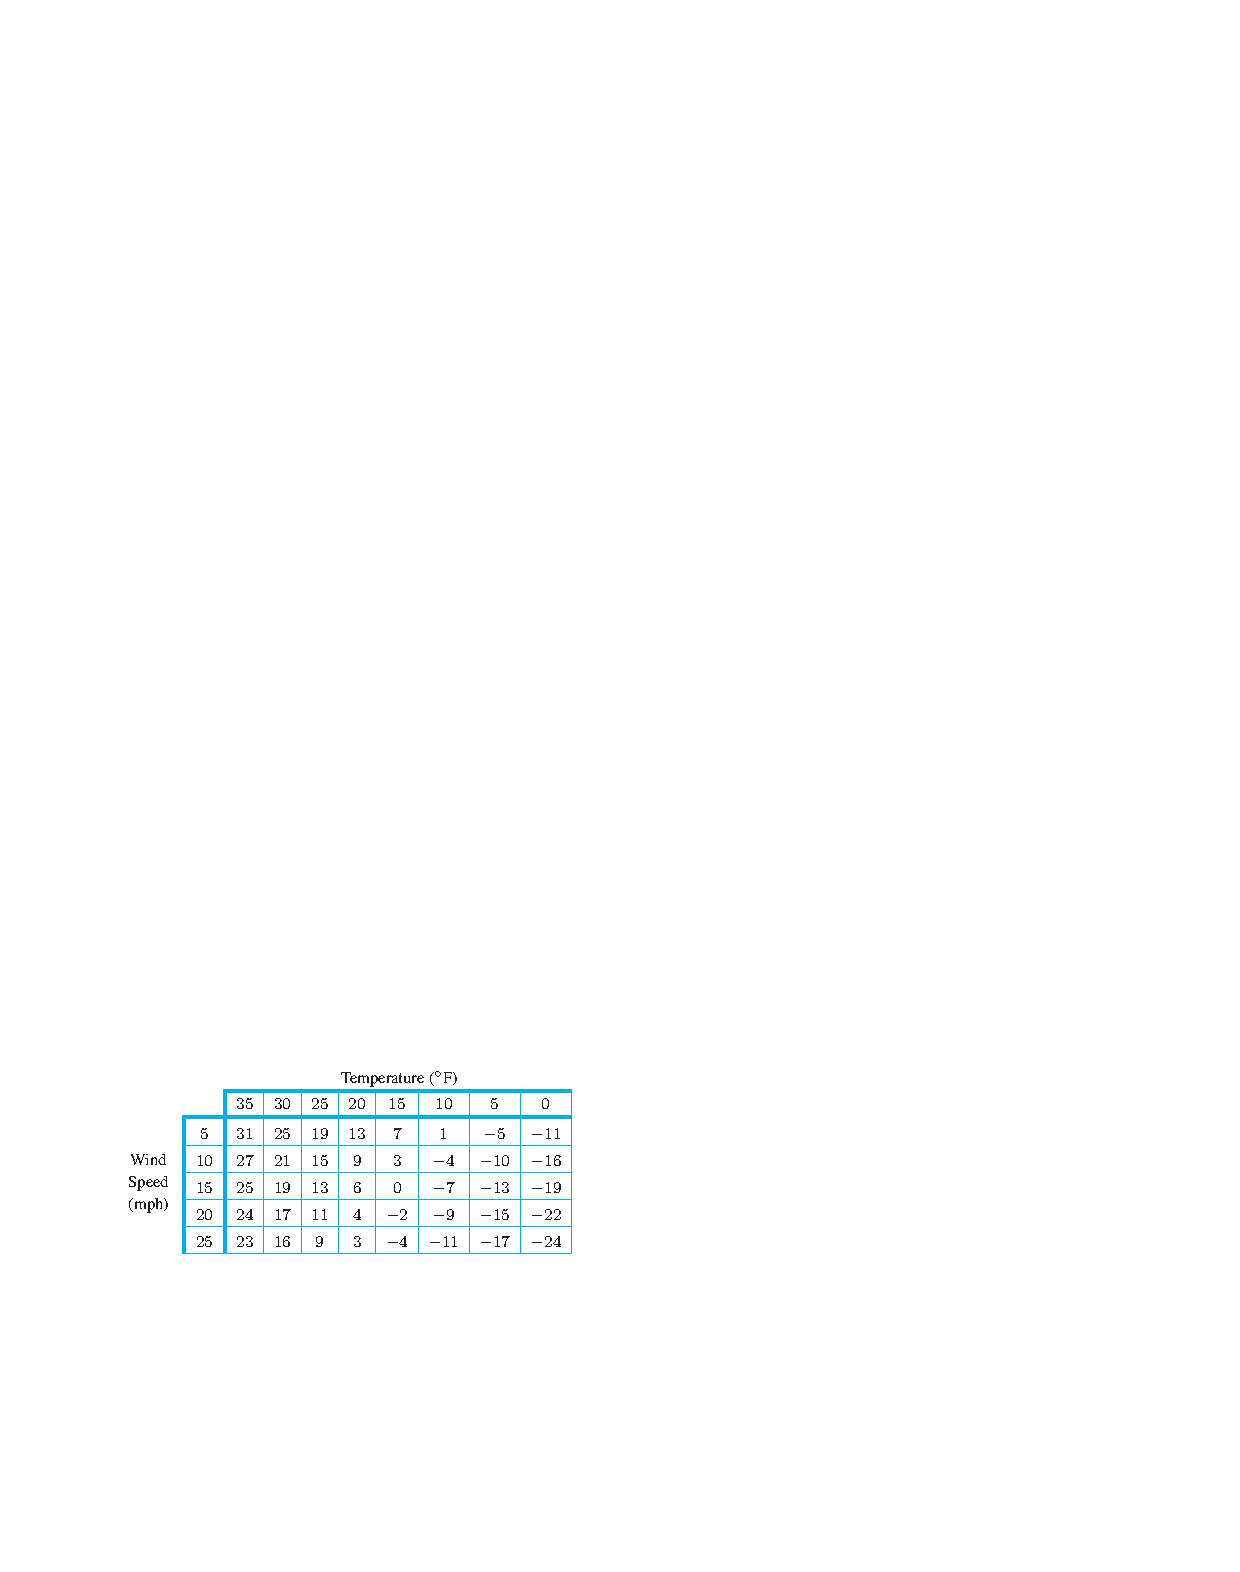
\includegraphics[scale=1]{1.pdf}
\end{center}
\medskip

\begin{enumerate}
\item Express the dependency of wind chill on wind and temperature in function notation.\vfill
\item If the temperature is $0^\circ$F and the wind speed is 15 mph, how cold does it feel?\vfill
\item If the temperature is $35^\circ$F, what wind speed makes it feel like $24^\circ$F?\vfill
\end{enumerate}

\prob A car rental company charges \$40 per day and 15 cents a mile for its cars.

\medskip
\begin{enumerate}
\item Write a formula for the cost, $C$, of renting a car as a function, $h$, of the number of days, $d$, and the number of miles driven, $m$.\vfill
\item Find $h(5,300)$ and interpret it.
\end{enumerate}

\vfill
\newpage
\prob Suppose $f(x,y) = x^2y + \sqrt{x}$.

\medskip
\begin{henumerate}{2}
\item $f(1,2)$
\item $f(9,4)$
\end{henumerate}

\vspace{1.5in}
\prob Consider the three points
\begin{align*}
A &= (1.3, -2.7,0), \\
B &= (0.9,0,3.2), \\
C &= (2.5,0.1,-0.3),
\end{align*}
in $\bbr^3$.

\medskip
\begin{enumerate}
\item Which one is closest to the $yz$-plane?\vfill
\item Which one lies on the $xy$-plane?\vfill
\item Which one is farthest from the $xz$-plane?\vfill
\end{enumerate}
\end{document}